% Section: Event generators and readers
\section{Event generators and readers}
\label{sec:generators}

Events are produced by generators, which simulate collisions, and by readers, which take them from files written by
other programs. Both are event processors (Section~\ref{sec:tasks}) that add particles to the events of the job; they
are placed in the event loop, as subtasks of an \code{EventIterator}, before the tasks that use their events. The
iterator resets the events before each pass and the generators only add to them, so that several generators can fill
one event, and \code{EventMerger} fills one event with several events of each of its input streams, to simulate
pile-up or to embed a hard process in a soft background. A reader ends the event loop when its input is exhausted.
The particles are created by the particle factory of the job and typed by the particle database of the task
(\code{PARTICLE\_DB}), so that the analyses see the same particle types whatever the source of the events; the
unstable particles that a generator emits are decayed, when they are, by the generator itself or by
\code{ParticleDecayerTask}, which follows the decay modes and branching ratios of the database through two-, three-
and four-body decays and decays the products in turn.

% ---------------------------------------------------------------------------------------------------------------
\subsection{BasicEventGen}
\label{sec:basicgen}

\code{BasicEventGen} is a fast generator of simple events, meant for tests and demonstrations of the analyses rather
than for physics: its particles are independent, without correlations, and emitted at the origin. The particle types
are given by their PDG codes (\code{PdgSelected}, e.g.\ \code{211, -211, 321, -321}), and the number of particles of
each type in an event is drawn uniformly between \code{MultMin} and \code{MultMax}. The momenta are generated in one
of two styles (\code{EventGenType}):
\begin{itemize}
  \item cylindrical (0): the rapidity is uniform between \code{RapidityMin} and \code{RapidityMax}, the azimuth uniform
  between \code{PhiMin} and \code{PhiMax}, and the transverse momentum is drawn from the momentum distribution,
  either within a range of transverse momentum, \code{PtMin} to \code{PtMax}, or within a range of momentum,
  \code{PMin} to \code{PMax} (\code{MomentumRange} = \code{PT} or \code{P});
  \item spherical (1): the momentum is drawn from the momentum distribution between \code{PMin} and \code{PMax}, the
  polar angle isotropically (uniform $\cos\theta$) between \code{ThetaMin} and \code{ThetaMax}, and the azimuth
  uniformly.
\end{itemize}
The momentum distribution, $dN/dx$ with $x = \pT$ or $p$ (\code{Distribution}), is an exponential,
$e^{-x/\lambda}$ (slope $\lambda$ = \code{Slope}, 0.5~GeV/$c$ by default), a Gaussian centred at zero,
$e^{-x^2/2\sigma^2}$ (\code{Sigma}), or any function of one variable of the function registry
(Section~\ref{sec:functions}), named by \code{Function:Name} with its parameters in \code{Function:Parameters}: a
registered class, such as \code{Exponential} or \code{Polynomial}, or a composite built in CapGui. The Gaussian and
the functions are tabulated on the range when the task is initialised and sampled by inverting their cumulative.
New styles of generation are added as new values of \code{EventGenType}. For tests of flow analyses
(Section~\ref{sec:flow}), \code{Flow:Vn} lists coefficients $v_1, v_2, \dots$ that modulate the azimuths about a
reaction plane $\Psi$ drawn for each event, $dN/d\varphi \propto 1 + 2\sum_n v_n(\pT)\cos n(\varphi-\Psi)$, with
$v_n(\pT) = v_n$, or $v_n\min(\pT/p_0,1)$ for $p_0$ = \code{Flow:PtScale}; the azimuths are drawn by rejection. The
random numbers are drawn by a Mersenne Twister, with the seed \code{Random:Seed}.

% ---------------------------------------------------------------------------------------------------------------
\subsection{Therminator3}
\label{sec:therminator}

\paragraph{Origin.}
Therminator3 is the thermal generator of \CAP{}. It is based on THERMINATOR~2~\cite{Chojnacki:2011hb} (release 2.0.3),
itself an extension of THERMINATOR~\cite{Kisiel:2005hn}, by M.~Chojnacki, A.~Kisiel, W.~Broniowski and W.~Florkowski,
from which it takes its physics: the statistical emission of hadrons from a freeze-out hypersurface, the freeze-out
models, the format of the hydrodynamic hypersurfaces, and the method of generation. The code was redesigned for
\CAP{}: the class structure is simplified, the configuration files of THERMINATOR~2 are replaced by the configuration
keys of a task, its ROOT data structures by the scalar fields, particles and events of \CAP{}, and its particle tables
by the particle database of \CAP{}; the decays of the resonances and the analysis of the events are left to the
other tasks of the job.

\paragraph{Class structure.}
The task \code{Therminator3} owns a freeze-out model, a class derived from \code{Model}. \code{Model} gathers the
settings of a model (\code{ModelSettings}), the thermodynamic fields of the freeze-out (\code{Thermodynamics}: the
temperature and, through \code{Chemistry}, the chemical potentials, uniform or varying across the hypersurface), the
geometry of the hypersurface (\code{Hypersurface}), and the hadron gas to emit (\code{ThermalHadronGas}). A model
implements one function, the integrand of the Cooper--Frye formula for a hadron at a point of the hypersurface and a
momentum, both drawn at random; everything else, the integration of the multiplicities and the generation of the
events, is done by \code{Model}. The fields read from hypersurface files are \code{ScalarField} objects of the Math
library (Section~\ref{sec:functions}). Figure~\ref{fig:therminator} shows the classes of the folder.

\begin{figure*}[t]
  \centering
  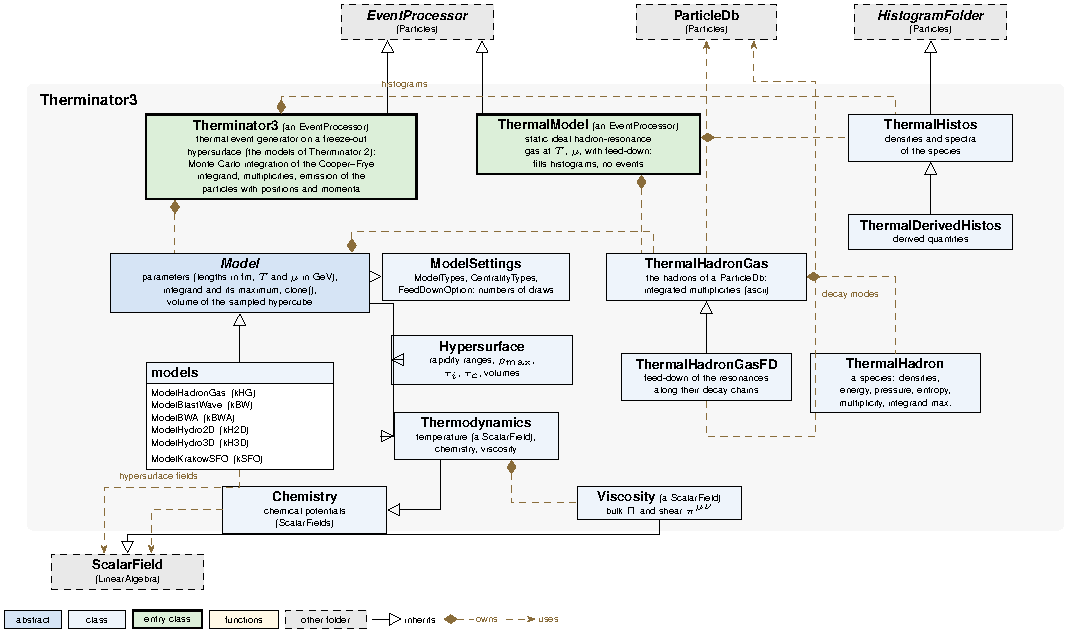
\includegraphics[width=\textwidth]{Therminator3Classes}
  \caption{Classes of Therminator3 (\code{models/Therminator3}): the generator task, the freeze-out models, the thermodynamic fields, the hadron gas, and the thermal model. Boxes: abstract classes (blue), classes (light blue), the entry classes of the folder (green), free functions (yellow), classes of other folders (grey, dashed). Open triangles point to the base class; dashed lines are dependencies, the diamond marking the owner.}
  \label{fig:therminator}
\end{figure*}

\paragraph{Emission.}
Hadrons are emitted according to the Cooper--Frye formula,
\begin{align}
  E\frac{dN}{d^3p} & = \frac{g}{(2\pi)^3}\int_\Sigma d\Sigma_\mu(x)\,p^\mu f(x,p), \\
  f(x,p) & = \frac{1}{\exp\!\bigl[(p\cdot u(x) - \mu(x))/T(x)\bigr] \pm 1},
\end{align}
with Fermi--Dirac or Bose--Einstein statistics, where $u$ is the velocity of the fluid on the hypersurface $\Sigma$, $T$
its temperature, and $\mu = B\mu_B + I_3\mu_I + S\mu_S + C\mu_C$ the chemical potential of the hadron, of baryon number
$B$, isospin $I_3$, strangeness $S$ and charm $C$. The hadrons emitted are those of the particle database, except the
quarks, leptons and gauge bosons and the hadrons heavier than 2.5~GeV; photons are not emitted.

\paragraph{Generation.}
As in THERMINATOR~2, the generation has two steps. First, the mean multiplicity $\avg{N}$ of each hadron is the
integral of the Cooper--Frye formula over the hypersurface and the momenta, computed by Monte Carlo
(\code{NSamples} points, $10^5$ by default), which also gives the maximum of the integrand. Then, for each event, the
number of each hadron is drawn from a Poisson distribution of mean $\avg{N}$ (or a Gaussian, \code{FluctuationType}),
and each hadron is generated by accepting or rejecting points of the integrand, drawn at random, against its maximum
times a safety factor (\code{MaxIntegrandSafety}, 1.2): the accepted point gives both the momentum of the hadron and
its position of emission, in fm. The multiplicities can be written to a file and read back, so that the integration
is done once for a set of parameters. The hadrons are emitted as they are produced, resonances included; a
\code{ParticleDecayerTask} placed after Therminator3 decays them.

\paragraph{Freeze-out models.}
The model is chosen by the key \code{HYDRO\_MODEL:TYPE}. All models share the sampling of the integrand. A point of
the hypersurface is drawn uniformly in the coordinates that parametrise it, and the momentum is drawn as
$\pT = \zeta/(1-\zeta)$ with $\zeta$ uniform in $[0,1)$, the rapidity $y$ uniform over a range $Y$
(\code{pRapidityRange}), and the azimuth $\varphi_p$ uniform. The integrand is then
\begin{equation}
  I = \frac{g}{(2\pi)^3}\,\frac{\pT}{(1-\zeta)^2}\,(d\Sigma\cdot p)\,f(x,p),
  \label{eq:t3-integrand}
\end{equation}
where $1/(1-\zeta)^2 = d\pT/d\zeta$, $p = (m_T\cosh y,\ \pT\cos\varphi_p,\ \pT\sin\varphi_p,\ m_T\sinh y)$ and $m_T = \sqrt{m^2+\pT^2}$. The mean
multiplicity is $\avg{N} = V\avg{I}$, where $V$ is the volume of the sampled region of coordinates and momenta. The
models differ by the hypersurface, the measure $d\Sigma\cdot p$ and the fluid velocity $u$ that enters $p\cdot u$.
Positions are written as $x = (\tau\cosh\eta,\ \rho\cos\varphi,\ \rho\sin\varphi,\ \tau\sinh\eta)$, with the
spatial rapidity $\eta$ uniform over \code{sRapidityRange}.
\begin{itemize}
  \item \code{BW}, the blast wave. Emission occurs at a constant proper time $\tau$ (\code{TauI}) from a cylinder of radius
  $\rho_{\max}$, with a radial transverse velocity $v_T$ (\code{tVelocity}) that is the same everywhere:
  \begin{align}
    p\cdot u & = \gamma_T\bigl(m_T\cosh(\eta-y) \nonumber\\ & \quad - v_T\pT\cos(\varphi-\varphi_p)\bigr), \\
    d\Sigma\cdot p & = \tau\rho\, m_T\cosh(\eta-y),
  \end{align}
  with $\gamma_T = (1-v_T^2)^{-1/2}$.
  \item \code{HG}, a static fireball: the blast wave without flow, $v_T = 0$.
  \item \code{BWA}, the variants of the blast wave of THERMINATOR~2 (\code{Subtype} 2 to 6). The hypersurface is tilted
  in the $(\tau,\rho)$ plane, $\tau(\rho) = \tau_i + A\rho$ (\code{Amplitude}), so that
  \begin{equation}
    d\Sigma\cdot p = \tau\rho\bigl(m_T\cosh(\eta-y) - A\,\pT\cos(\varphi-\varphi_p)\bigr).
  \end{equation}
  The transverse velocity is either constant (subtypes 2 and 3) or rises with the radius as
  $v_T(\rho) = (\rho/\rho_{\max})/(v + \rho/\rho_{\max})$, with $v$ = \code{tVelocity} (subtypes 4 to 6; Eq.~(42) of
  Ref.~\cite{Chojnacki:2011hb}). In subtypes 3, 5 and 6 the emission is delayed by a time $\Delta$ drawn from an
  exponential distribution of mean \code{Delay}. In subtype 6, which is new in \CAP{}, the particle also streams
  freely during the delay, $\vec{x} \to \vec{x} + \Delta\,\vec{p}/E$.
  \item \code{SFO}, the Krak\'ow single freeze-out model~\cite{Broniowski:2001we}. Emission occurs on the hyperboloid
  $\tau^2 - \rho^2 = \tau_f^2$ (\code{TauC}), with the Hubble-like flow $u = x/\tau_f$ of the single freeze-out:
  \begin{align}
    p\cdot u & = \frac{m_T\,\tau\cosh(\eta-y) - \pT\rho\cos(\varphi-\varphi_p)}{\tau_f}, \\
    d\Sigma\cdot p & = \tau_f\,\rho\,(p\cdot u),
  \end{align}
  where $\tau = \sqrt{\tau_f^2+\rho^2}$ is the proper time of the emission point.
  \item \code{HYDRO2D}, a hypersurface of boost-invariant (2+1)-dimensional hydrodynamics. The surface is the distance
  $D(\zeta,\varphi)$ from the point $(\tau_i, 0)$ of the $(\tau,\rho)$ plane, so that $\tau = \tau_i + D\sin\zeta$ and
  $\rho = D\cos\zeta$. The fluid has a transverse velocity $v_T(\zeta,\varphi)$ at an azimuth $\varphi + \varphi_F$, and
  \begin{align}
    p\cdot u & = \gamma_T\bigl(m_T\cosh(y-\eta) \nonumber\\ & \quad - v_T\pT\cos(\varphi-\varphi_p+\varphi_F)\bigr), \\
    d\Sigma\cdot p & = D\,\tau\,\bigl[D\cos\zeta\,(m_T\sin\zeta\,C + \pT\cos\zeta\,c) \nonumber\\
    & \quad + \partial_\zeta D\,\cos\zeta\,(\pT\sin\zeta\,c - m_T\cos\zeta\,C) \nonumber\\
    & \quad + \partial_\varphi D\,\pT\,s\bigr],
  \end{align}
  with $C = \cosh(y-\eta)$, $c = \cos(\varphi-\varphi_p)$ and $s = \sin(\varphi-\varphi_p)$.
  \item \code{HYDRO3D}, a hypersurface of (3+1)-dimensional hydrodynamics. The parametrisation adds a polar angle
  $\theta$: $\tau = \tau_i + D\sin\theta\sin\zeta$, $\rho = D\sin\theta\cos\zeta$, and $\eta = D\cos\theta/\Lambda$. The
  fluid has transverse components $u_x$, $u_y$ and a longitudinal rapidity $Y_F$, so that
  \begin{align}
    p\cdot u & = \sqrt{1+u_x^2+u_y^2}\; m_T\cosh(Y_F-y) \nonumber\\
    & \quad - \pT\,(u_x\cos\varphi_p + u_y\sin\varphi_p),
  \end{align}
  and $d\Sigma\cdot p$ follows from the derivatives of $D$ with respect to the three angles (Ref.~\cite{Chojnacki:2011hb}).
\end{itemize}
In the hydrodynamic models a negative $d\Sigma\cdot p$, a particle entering the hypersurface, is set to zero, as is
common practice; with \code{BackFlow}, only those particles are kept. The parameters of the analytic models
(temperature, chemical potentials, radius, proper times, velocity, ranges of rapidity) are keys of the task, with
lengths in fm and temperatures and chemical potentials in GeV; their defaults are those of the blast wave of
THERMINATOR~2. The hydrodynamic hypersurfaces are read from the XML files of THERMINATOR~2: the distance $D$ and the
fluid velocity as functions of the angles, together with the temperature, chemical potentials and initial proper time
of the calculation, which override those of the configuration. The derivatives of the distance are read when the file
provides them, and computed otherwise.
\todo{the shear and bulk viscous corrections ($\delta f$, class \code{Viscosity}) and the negative-binomial
fluctuations of the multiplicities are not finished; describe them when they are.}

\paragraph{Validation and the thermal model.}
The tests of Therminator3 compare its mean multiplicities of pions, kaons, protons and $\Lambda$ for the blast wave
with those of THERMINATOR~2 (agreement within 2.5\%), and the multiplicities and mean $\pT$ of generated events
with their expected values; they check that hydrodynamic hypersurfaces built to equal the blast wave reproduce its
multiplicities, in 2+1 and 3+1 dimensions, and, when THERMINATOR~2 is installed, run a hypersurface of its library.
A second task, \code{ThermalModel}, computes the densities, energy densities, pressures and entropy densities of a
static ideal hadron-resonance gas at a given temperature and chemical potentials, with the feed-down of the
resonances to the stable hadrons through their decays, and fills histograms of them; it generates no events.
The densities are the series
$n = \frac{g\,m^2T}{2\pi^2}\sum_{k\ge1}(\mp1)^{k+1}\lambda^k K_2(km/T)/k$, with the fugacity $\lambda = e^{\mu/T}$ and the
upper sign for fermions, truncated at five terms. The feed-down to a stable hadron follows the decay chains of the
particle database, with the branching ratios normalized to one, as the decayer draws them.
\todo{$\mu_Q$ is not used by \code{ThermalHadron::calculateAllProperties}: add it or remove the key.}

% ---------------------------------------------------------------------------------------------------------------
\subsection{Pythia8}
\label{sec:pythia}

\code{PythiaEventGenerator} generates events with Pythia~8~\cite{Bierlich:2022pfr}, linked to \CAP{} when it is built
with Pythia (Section~\ref{sec:build}). The beams are set by their PDG codes and either the energy in the centre of mass
or the energies of the two beams (proton--proton at 2.7~TeV by default), and the seed by \code{SeedValue}. Three
presets set the many Pythia parameters of models of collective effects in small systems: QCD-based colour
reconnection (\code{UseQCDCR}, on by default), rope hadronisation (\code{UseRopes}) and string shoving
(\code{UseShoving}). Any other Pythia setting is passed verbatim, as a string, by the keys \code{Option0} to
\code{Option29}, applied after the presets so that they can modify them. The particles of each Pythia event are
copied into the event of the task with their momenta and production vertices: by default the final-state particles
only, without photons, neutrinos, quarks, gluons and gauge bosons, each of which can be kept on request. Decays are
those of Pythia, set by its own options. The particles whose PDG code is not in the particle database of \CAP{} are
skipped and counted.

% ---------------------------------------------------------------------------------------------------------------
\subsection{Herwig 7}
\label{sec:herwig}

\code{HerwigEventGenerator} runs Herwig~7~\cite{Bellm:2015jjp} in the job, linked to \CAP{} when it is built with
Herwig (Section~\ref{sec:external}). Herwig is configured as on its command line: \code{Herwig read} turns an input
file (\code{.in}) of repository commands into a run file (\code{.run}) holding the event generator, and \code{Herwig
run} generates its events. The task does both. Given an input file (\code{InputFile}, or a \code{.in} file given as
\code{RunFile}), it reads it, in the directory of the file and with the repository \code{Repository}
(\code{HerwigDefaults.rpo} by default), unless the run file that the input saves is already there and is newer;
otherwise it loads the run file \code{RunFile}. Commands applied to the generator before the run, as by \code{Herwig
run -x}, come from a file (\code{SetupFile}) and from the keys \code{Option0} to \code{Option19}, for instance
{\small
\begin{verbatim}
set /Herwig/Generators/EventGenerator:
    EventHandler:LuminosityFunction:Energy 13600.0
set /Herwig/Particles/pi0:Stable Stable
\end{verbatim}
}
so that the beam energy, or the decays, can be changed without a new run file. The seed is set by \code{SeedValue}
(with \code{SetSeed}), and \code{Tag} is appended to the names of the log and output files that Herwig writes.
Processes integrated by Matchbox need their grids first, made by \code{Herwig build} and \code{Herwig integrate} on
the command line. Each Herwig event is generated by \code{execute()}, and its final-state particles are copied into
the event of the task with their momenta (GeV) and production vertices (mm): photons and neutrinos are included unless
\code{SavePhotons} or \code{SaveNeutrinos} is off, and a particle is added when it passes the first particle filter of
the task. As for Pythia, the particles whose PDG code is not in the particle database are skipped and counted.
Herwig's events are unweighted by default; weighted events, whose weight \CAP{} events cannot carry, are counted and
reported, together with the events that Herwig failed to generate. At the end of the job, the task reports the cross
section and Herwig writes its output file. Since Herwig keeps a global state, a job has a single
\code{HerwigEventGenerator}. On macOS, Herwig and ThePEG must be built with \code{-fno-typed-cxx-new-delete} and linked
to \code{libc++}, as is the \CAP{} module.

% ---------------------------------------------------------------------------------------------------------------
\subsection{Event readers}
\label{sec:readers}

Readers take the events produced by other generators from their files, found from the key \code{DataImportPath}
(the environment variable \code{CAP\_DATA\_IMPORT\_PATH} by default) and the name or pattern \code{DataImportFile}.
Particles whose PDG code is not in the particle database are skipped, and counted in the report of the task at the
end of the job.
\begin{itemize}
  \item \code{PythiaEventReader} reads Pythia events stored in ROOT trees of \code{TParticle} objects (key
  \code{TreeName}), a set of files being read as one chain; the particles kept are selected as by the generator.
  \item \code{EposEventReader} reads the ROOT trees written by EPOS~\cite{Werner:2010aa} (key \code{TreeName}), a set
  of files being read as one chain: per event, the number of particles, the impact parameter, and the PDG codes and
  momenta of the particles, whose energies are computed from the masses of the database.
  \item \code{PHSDEventReader} reads the text files of PHSD~\cite{Cassing:2009vt}: a file, or the files matching
  \code{DataImportFile} (\code{*.dat} by default) in a directory and its sub-directories, read in order. Each event
  has a header with the impact parameter, the colliding nuclei, the energy, the number of participants and the
  event-plane angles and eccentricities of orders 2 to 5, followed by the PDG codes, charges, momenta and energies of
  the particles; the particles keep the energies of the file, since PHSD particles may be off their mass shell.
\end{itemize}
\todo{the program writing the Pythia ROOT trees read by \code{PythiaEventReader} is not part of \CAP{}: say where
it comes from.}

% ---------------------------------------------------------------------------------------------------------------
\subsection{Glauber model}
\label{sec:glauber}

\paragraph{Class structure.}
The Monte Carlo Glauber model~\cite{Miller:2007ri} of \CAP{} derives from TGlauberMC, the PHOBOS Glauber Monte
Carlo~\cite{Alver:2008aq}. The task \code{GlauberGenerator} makes the events: for each event, it places the
nucleons of the two nuclei (\code{GlauberNucleus}, of a type \code{GlauberNucleusType} taken from the database
\code{GlauberDb}, with the radial densities of \code{NuclearDistribution}), draws the impact parameter, and finds
the binary and hard nucleon--nucleon collisions, with the collision profiles (\code{NNProfile},
\code{NucleonProfile}, \code{SmearingProfile}, \code{PTotProfile}) and the inelastic cross section
(\code{NNXSectVsSqrtS}). An event (\code{GlauberEvent}) holds the two nuclei, the impact parameter and the numbers
of participants, binary collisions and spectators. The task \code{GlauberAnalyzer} computes the moments of the
participants (\code{GlauberEventMoments}) and fills the histograms of \code{GlauberHistos} for each event filter
(\code{GlauberEventFilter}). Figure~\ref{fig:glauber} shows the classes of the folder.

\begin{figure*}[t]
  \centering
  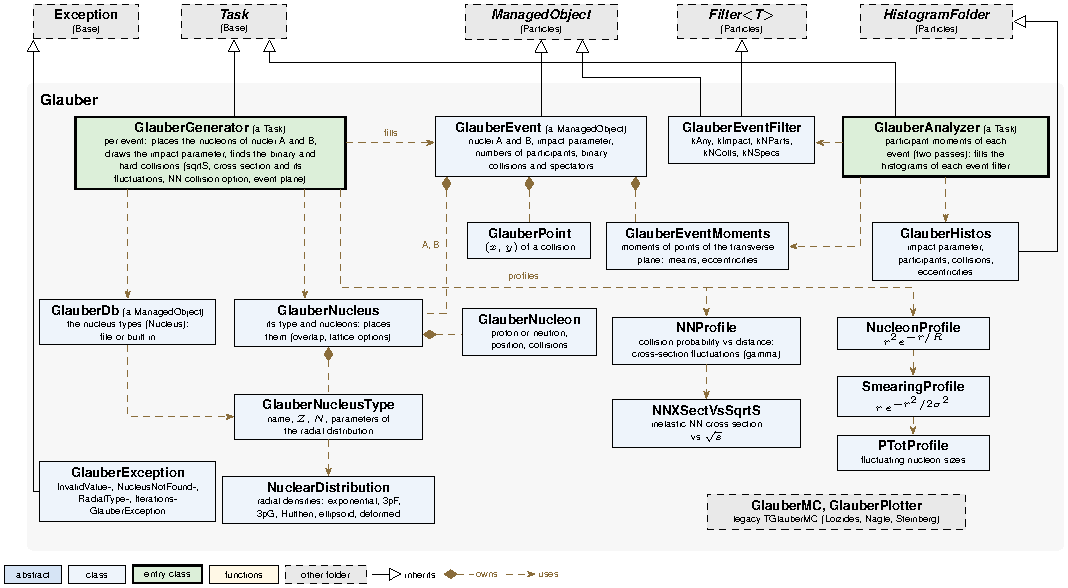
\includegraphics[width=\textwidth]{GlauberClasses}
  \caption{Classes of the Glauber model (\code{models/Glauber}). Boxes: abstract classes (blue), classes (light blue), the entry classes of the folder (green), free functions (yellow), classes of other folders (grey, dashed). Open triangles point to the base class; dashed lines are dependencies, the diamond marking the owner.}
  \label{fig:glauber}
\end{figure*}

\todo{to come later: event generation and analysis.}
